% Created by tikzDevice version 0.10.1 on 2016-08-02 15:11:32
% !TEX encoding = UTF-8 Unicode
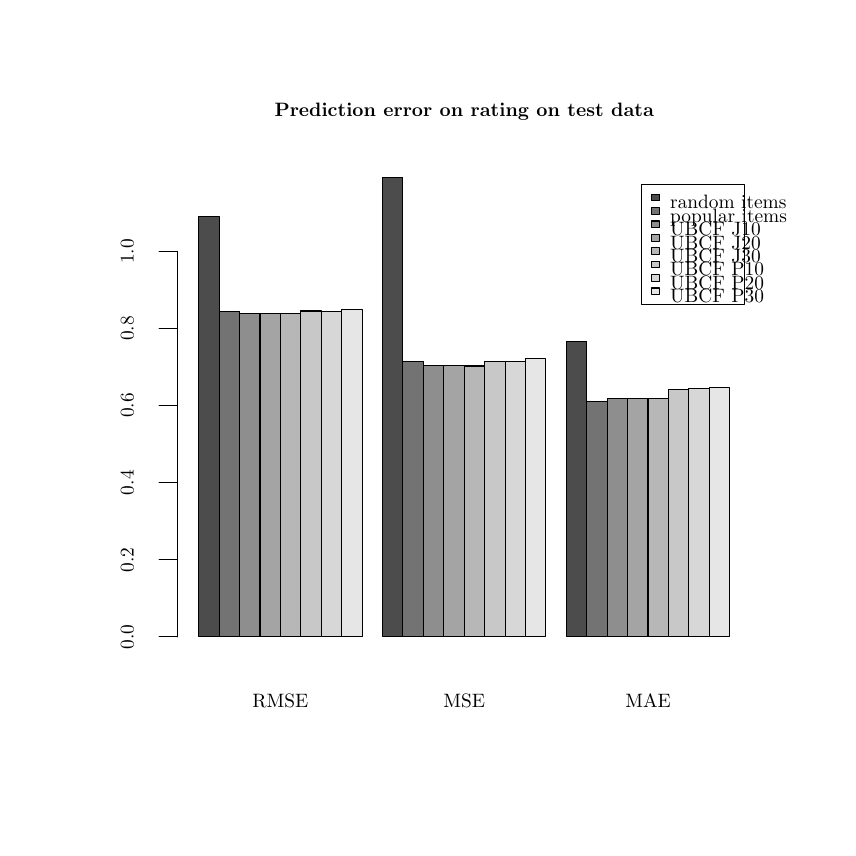
\begin{tikzpicture}[x=1pt,y=1pt]
\definecolor{fillColor}{RGB}{255,255,255}
\path[use as bounding box,fill=fillColor,fill opacity=0.00] (0,0) rectangle (289.08,289.08);
\begin{scope}
\path[clip] (  0.00,  0.00) rectangle (289.08,289.08);
\definecolor{drawColor}{RGB}{0,0,0}
\definecolor{fillColor}{gray}{0.30}

\path[draw=drawColor,line width= 0.4pt,line join=round,line cap=round,fill=fillColor] ( 61.80, 68.98) rectangle ( 69.18,221.00);
\definecolor{fillColor}{gray}{0.45}

\path[draw=drawColor,line width= 0.4pt,line join=round,line cap=round,fill=fillColor] ( 69.18, 68.98) rectangle ( 76.56,186.67);
\definecolor{fillColor}{RGB}{142,142,142}

\path[draw=drawColor,line width= 0.4pt,line join=round,line cap=round,fill=fillColor] ( 76.56, 68.98) rectangle ( 83.94,185.75);
\definecolor{fillColor}{RGB}{164,164,164}

\path[draw=drawColor,line width= 0.4pt,line join=round,line cap=round,fill=fillColor] ( 83.94, 68.98) rectangle ( 91.32,185.72);
\definecolor{fillColor}{RGB}{183,183,183}

\path[draw=drawColor,line width= 0.4pt,line join=round,line cap=round,fill=fillColor] ( 91.32, 68.98) rectangle ( 98.70,185.69);
\definecolor{fillColor}{RGB}{200,200,200}

\path[draw=drawColor,line width= 0.4pt,line join=round,line cap=round,fill=fillColor] ( 98.70, 68.98) rectangle (106.08,186.71);
\definecolor{fillColor}{RGB}{215,215,215}

\path[draw=drawColor,line width= 0.4pt,line join=round,line cap=round,fill=fillColor] (106.08, 68.98) rectangle (113.46,186.67);
\definecolor{fillColor}{RGB}{230,230,230}

\path[draw=drawColor,line width= 0.4pt,line join=round,line cap=round,fill=fillColor] (113.46, 68.98) rectangle (120.84,187.27);
\definecolor{fillColor}{gray}{0.30}

\path[draw=drawColor,line width= 0.4pt,line join=round,line cap=round,fill=fillColor] (128.22, 68.98) rectangle (135.60,234.96);
\definecolor{fillColor}{gray}{0.45}

\path[draw=drawColor,line width= 0.4pt,line join=round,line cap=round,fill=fillColor] (135.60, 68.98) rectangle (142.98,168.46);
\definecolor{fillColor}{RGB}{142,142,142}

\path[draw=drawColor,line width= 0.4pt,line join=round,line cap=round,fill=fillColor] (142.98, 68.98) rectangle (150.36,166.90);
\definecolor{fillColor}{RGB}{164,164,164}

\path[draw=drawColor,line width= 0.4pt,line join=round,line cap=round,fill=fillColor] (150.36, 68.98) rectangle (157.74,166.85);
\definecolor{fillColor}{RGB}{183,183,183}

\path[draw=drawColor,line width= 0.4pt,line join=round,line cap=round,fill=fillColor] (157.74, 68.98) rectangle (165.12,166.81);
\definecolor{fillColor}{RGB}{200,200,200}

\path[draw=drawColor,line width= 0.4pt,line join=round,line cap=round,fill=fillColor] (165.12, 68.98) rectangle (172.50,168.52);
\definecolor{fillColor}{RGB}{215,215,215}

\path[draw=drawColor,line width= 0.4pt,line join=round,line cap=round,fill=fillColor] (172.50, 68.98) rectangle (179.88,168.46);
\definecolor{fillColor}{RGB}{230,230,230}

\path[draw=drawColor,line width= 0.4pt,line join=round,line cap=round,fill=fillColor] (179.88, 68.98) rectangle (187.26,169.47);
\definecolor{fillColor}{gray}{0.30}

\path[draw=drawColor,line width= 0.4pt,line join=round,line cap=round,fill=fillColor] (194.64, 68.98) rectangle (202.02,175.73);
\definecolor{fillColor}{gray}{0.45}

\path[draw=drawColor,line width= 0.4pt,line join=round,line cap=round,fill=fillColor] (202.02, 68.98) rectangle (209.40,154.01);
\definecolor{fillColor}{RGB}{142,142,142}

\path[draw=drawColor,line width= 0.4pt,line join=round,line cap=round,fill=fillColor] (209.40, 68.98) rectangle (216.78,155.16);
\definecolor{fillColor}{RGB}{164,164,164}

\path[draw=drawColor,line width= 0.4pt,line join=round,line cap=round,fill=fillColor] (216.78, 68.98) rectangle (224.16,155.15);
\definecolor{fillColor}{RGB}{183,183,183}

\path[draw=drawColor,line width= 0.4pt,line join=round,line cap=round,fill=fillColor] (224.16, 68.98) rectangle (231.54,155.16);
\definecolor{fillColor}{RGB}{200,200,200}

\path[draw=drawColor,line width= 0.4pt,line join=round,line cap=round,fill=fillColor] (231.54, 68.98) rectangle (238.92,158.38);
\definecolor{fillColor}{RGB}{215,215,215}

\path[draw=drawColor,line width= 0.4pt,line join=round,line cap=round,fill=fillColor] (238.92, 68.98) rectangle (246.30,158.68);
\definecolor{fillColor}{RGB}{230,230,230}

\path[draw=drawColor,line width= 0.4pt,line join=round,line cap=round,fill=fillColor] (246.30, 68.98) rectangle (253.68,159.07);
\end{scope}
\begin{scope}
\path[clip] (  0.00,  0.00) rectangle (289.08,289.08);
\definecolor{drawColor}{RGB}{0,0,0}

\node[text=drawColor,anchor=base,inner sep=0pt, outer sep=0pt, scale=  0.7] at ( 91.32, 43.56) {RMSE};

\node[text=drawColor,anchor=base,inner sep=0pt, outer sep=0pt, scale=  0.7] at (157.74, 43.56) {MSE};

\node[text=drawColor,anchor=base,inner sep=0pt, outer sep=0pt, scale=  0.7] at (224.16, 43.56) {MAE};
\end{scope}
\begin{scope}
\path[clip] (  0.00,  0.00) rectangle (289.08,289.08);
\definecolor{drawColor}{RGB}{0,0,0}
\definecolor{fillColor}{RGB}{255,255,255}

\path[draw=drawColor,line width= 0.4pt,line join=round,line cap=round,fill=fillColor] (221.77,232.54) rectangle (258.89,188.96);
\definecolor{fillColor}{gray}{0.30}

\path[draw=drawColor,line width= 0.4pt,line join=round,line cap=round,fill=fillColor] (225.47,228.91) rectangle (228.43,226.49);
\definecolor{fillColor}{gray}{0.45}

\path[draw=drawColor,line width= 0.4pt,line join=round,line cap=round,fill=fillColor] (225.47,224.06) rectangle (228.43,221.64);
\definecolor{fillColor}{RGB}{142,142,142}

\path[draw=drawColor,line width= 0.4pt,line join=round,line cap=round,fill=fillColor] (225.47,219.22) rectangle (228.43,216.80);
\definecolor{fillColor}{RGB}{164,164,164}

\path[draw=drawColor,line width= 0.4pt,line join=round,line cap=round,fill=fillColor] (225.47,214.38) rectangle (228.43,211.96);
\definecolor{fillColor}{RGB}{183,183,183}

\path[draw=drawColor,line width= 0.4pt,line join=round,line cap=round,fill=fillColor] (225.47,209.54) rectangle (228.43,207.12);
\definecolor{fillColor}{RGB}{200,200,200}

\path[draw=drawColor,line width= 0.4pt,line join=round,line cap=round,fill=fillColor] (225.47,204.70) rectangle (228.43,202.27);
\definecolor{fillColor}{RGB}{215,215,215}

\path[draw=drawColor,line width= 0.4pt,line join=round,line cap=round,fill=fillColor] (225.47,199.85) rectangle (228.43,197.43);
\definecolor{fillColor}{RGB}{230,230,230}

\path[draw=drawColor,line width= 0.4pt,line join=round,line cap=round,fill=fillColor] (225.47,195.01) rectangle (228.43,192.59);

\node[text=drawColor,anchor=base west,inner sep=0pt, outer sep=0pt, scale=  0.7] at (232.13,223.58) {random items};

\node[text=drawColor,anchor=base west,inner sep=0pt, outer sep=0pt, scale=  0.7] at (232.13,218.74) {popular items};

\node[text=drawColor,anchor=base west,inner sep=0pt, outer sep=0pt, scale=  0.7] at (232.13,213.90) {UBCF J10};

\node[text=drawColor,anchor=base west,inner sep=0pt, outer sep=0pt, scale=  0.7] at (232.13,209.06) {UBCF J20};

\node[text=drawColor,anchor=base west,inner sep=0pt, outer sep=0pt, scale=  0.7] at (232.13,204.21) {UBCF J30};

\node[text=drawColor,anchor=base west,inner sep=0pt, outer sep=0pt, scale=  0.7] at (232.13,199.37) {UBCF P10};

\node[text=drawColor,anchor=base west,inner sep=0pt, outer sep=0pt, scale=  0.7] at (232.13,194.53) {UBCF P20};

\node[text=drawColor,anchor=base west,inner sep=0pt, outer sep=0pt, scale=  0.7] at (232.13,189.69) {UBCF P30};
\end{scope}
\begin{scope}
\path[clip] (  0.00,  0.00) rectangle (289.08,289.08);
\definecolor{drawColor}{RGB}{0,0,0}

\path[draw=drawColor,line width= 0.4pt,line join=round,line cap=round] ( 54.12, 68.98) -- ( 54.12,208.22);

\path[draw=drawColor,line width= 0.4pt,line join=round,line cap=round] ( 54.12, 68.98) -- ( 47.52, 68.98);

\path[draw=drawColor,line width= 0.4pt,line join=round,line cap=round] ( 54.12, 96.83) -- ( 47.52, 96.83);

\path[draw=drawColor,line width= 0.4pt,line join=round,line cap=round] ( 54.12,124.67) -- ( 47.52,124.67);

\path[draw=drawColor,line width= 0.4pt,line join=round,line cap=round] ( 54.12,152.52) -- ( 47.52,152.52);

\path[draw=drawColor,line width= 0.4pt,line join=round,line cap=round] ( 54.12,180.37) -- ( 47.52,180.37);

\path[draw=drawColor,line width= 0.4pt,line join=round,line cap=round] ( 54.12,208.22) -- ( 47.52,208.22);

\node[text=drawColor,rotate= 90.00,anchor=base,inner sep=0pt, outer sep=0pt, scale=  0.7] at ( 38.28, 68.98) {0.0};

\node[text=drawColor,rotate= 90.00,anchor=base,inner sep=0pt, outer sep=0pt, scale=  0.7] at ( 38.28, 96.83) {0.2};

\node[text=drawColor,rotate= 90.00,anchor=base,inner sep=0pt, outer sep=0pt, scale=  0.7] at ( 38.28,124.67) {0.4};

\node[text=drawColor,rotate= 90.00,anchor=base,inner sep=0pt, outer sep=0pt, scale=  0.7] at ( 38.28,152.52) {0.6};

\node[text=drawColor,rotate= 90.00,anchor=base,inner sep=0pt, outer sep=0pt, scale=  0.7] at ( 38.28,180.37) {0.8};

\node[text=drawColor,rotate= 90.00,anchor=base,inner sep=0pt, outer sep=0pt, scale=  0.7] at ( 38.28,208.22) {1.0};
\end{scope}
\begin{scope}
\path[clip] (  0.00,  0.00) rectangle (289.08,289.08);
\definecolor{drawColor}{RGB}{0,0,0}

\node[text=drawColor,anchor=base,inner sep=0pt, outer sep=0pt, scale=  0.7] at (157.74,257.07) {\bfseries Prediction error on rating on test data};
\end{scope}
\end{tikzpicture}
